\hypertarget{_lgm___vec_8c}{
\section{/home/mgh/LanlGeoMag/libLanlGeoMag/Lgm\_\-Vec.c File Reference}
\label{_lgm___vec_8c}\index{/home/mgh/LanlGeoMag/libLanlGeoMag/Lgm\_\-Vec.c@{/home/mgh/LanlGeoMag/libLanlGeoMag/Lgm\_\-Vec.c}}
}
{\tt \#include $<$math.h$>$}\par
{\tt \#include \char`\"{}Lgm/Lgm\_\-Vec.h\char`\"{}}\par


Include dependency graph for Lgm\_\-Vec.c:\nopagebreak
\begin{figure}[H]
\begin{center}
\leavevmode
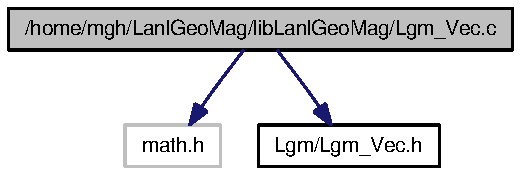
\includegraphics[width=143pt]{_lgm___vec_8c__incl}
\end{center}
\end{figure}
\subsection*{Functions}
\begin{CompactItemize}
\item 
\hyperlink{struct_lgm___vector}{Lgm\_\-Vector} $\ast$ \hyperlink{_lgm___vec_8c_208f75bd83a322d75a1e5f741bd73e34}{Lgm\_\-CreateVector} (double x, double y, double z)
\item 
void \hyperlink{_lgm___vec_8c_390e6254a5488b560011b0c1880745dd}{Lgm\_\-CrossProduct} (\hyperlink{struct_lgm___vector}{Lgm\_\-Vector} $\ast$a, \hyperlink{struct_lgm___vector}{Lgm\_\-Vector} $\ast$b, \hyperlink{struct_lgm___vector}{Lgm\_\-Vector} $\ast$c)
\item 
double \hyperlink{_lgm___vec_8c_bc4f50854f167ab190d1ec48cba5fb6f}{Lgm\_\-DotProduct} (\hyperlink{struct_lgm___vector}{Lgm\_\-Vector} $\ast$a, \hyperlink{struct_lgm___vector}{Lgm\_\-Vector} $\ast$b)
\item 
double \hyperlink{_lgm___vec_8c_851c60a1429e5b2d8bc5feb2d59af700}{Lgm\_\-NormalizeVector} (\hyperlink{struct_lgm___vector}{Lgm\_\-Vector} $\ast$a)
\item 
void \hyperlink{_lgm___vec_8c_eb74ea961a602bfdb729ade5b1282946}{Lgm\_\-ScaleVector} (\hyperlink{struct_lgm___vector}{Lgm\_\-Vector} $\ast$a, double value)
\item 
double \hyperlink{_lgm___vec_8c_84b4b9aa2d74211cb12654e6be70cb82}{Lgm\_\-Magnitude} (\hyperlink{struct_lgm___vector}{Lgm\_\-Vector} $\ast$a)
\item 
void \hyperlink{_lgm___vec_8c_59a0c49aecd33af604d43a47637bc281}{Lgm\_\-VecSub} (\hyperlink{struct_lgm___vector}{Lgm\_\-Vector} $\ast$c, \hyperlink{struct_lgm___vector}{Lgm\_\-Vector} $\ast$a, \hyperlink{struct_lgm___vector}{Lgm\_\-Vector} $\ast$b)
\item 
void \hyperlink{_lgm___vec_8c_3229855b208a924cdbab19bbb9df87d9}{Lgm\_\-VecAdd} (\hyperlink{struct_lgm___vector}{Lgm\_\-Vector} $\ast$c, \hyperlink{struct_lgm___vector}{Lgm\_\-Vector} $\ast$a, \hyperlink{struct_lgm___vector}{Lgm\_\-Vector} $\ast$b)
\item 
double \hyperlink{_lgm___vec_8c_3e1cdd838a8f00a41c167e848f6decf5}{Lgm\_\-VecDiffMag} (\hyperlink{struct_lgm___vector}{Lgm\_\-Vector} $\ast$a, \hyperlink{struct_lgm___vector}{Lgm\_\-Vector} $\ast$b)
\item 
void \hyperlink{_lgm___vec_8c_47c6f330f5c1228f812b005094b64dfd}{Lgm\_\-ForceMagnitude} (\hyperlink{struct_lgm___vector}{Lgm\_\-Vector} $\ast$a, double mag)
\item 
void \hyperlink{_lgm___vec_8c_d6b4ead73e36f4f3f77cc62bc88555d3}{Lgm\_\-MatTimesVec} (double A\mbox{[}3\mbox{]}\mbox{[}3\mbox{]}, \hyperlink{struct_lgm___vector}{Lgm\_\-Vector} $\ast$V, \hyperlink{struct_lgm___vector}{Lgm\_\-Vector} $\ast$Result)
\item 
void \hyperlink{_lgm___vec_8c_f287f148b722a2622150934c23fa59d4}{Lgm\_\-Transpose} (double A\mbox{[}3\mbox{]}\mbox{[}3\mbox{]}, double B\mbox{[}3\mbox{]}\mbox{[}3\mbox{]})
\item 
void \hyperlink{_lgm___vec_8c_cc29cb583eff692c2df92d9a49f3ce9e}{Lgm\_\-MatTimesMat} (double A\mbox{[}3\mbox{]}\mbox{[}3\mbox{]}, double B\mbox{[}3\mbox{]}\mbox{[}3\mbox{]}, double R\mbox{[}3\mbox{]}\mbox{[}3\mbox{]})
\end{CompactItemize}


\subsection{Function Documentation}
\hypertarget{_lgm___vec_8c_208f75bd83a322d75a1e5f741bd73e34}{
\index{Lgm\_\-Vec.c@{Lgm\_\-Vec.c}!Lgm\_\-CreateVector@{Lgm\_\-CreateVector}}
\index{Lgm\_\-CreateVector@{Lgm\_\-CreateVector}!Lgm_Vec.c@{Lgm\_\-Vec.c}}
\subsubsection[{Lgm\_\-CreateVector}]{\setlength{\rightskip}{0pt plus 5cm}{\bf Lgm\_\-Vector}$\ast$ Lgm\_\-CreateVector (double {\em x}, \/  double {\em y}, \/  double {\em z})}}
\label{_lgm___vec_8c_208f75bd83a322d75a1e5f741bd73e34}




Definition at line 7 of file Lgm\_\-Vec.c.

Here is the caller graph for this function:\nopagebreak
\begin{figure}[H]
\begin{center}
\leavevmode
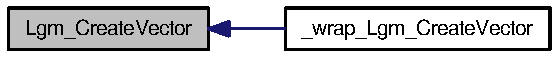
\includegraphics[width=152pt]{_lgm___vec_8c_208f75bd83a322d75a1e5f741bd73e34_icgraph}
\end{center}
\end{figure}
\hypertarget{_lgm___vec_8c_390e6254a5488b560011b0c1880745dd}{
\index{Lgm\_\-Vec.c@{Lgm\_\-Vec.c}!Lgm\_\-CrossProduct@{Lgm\_\-CrossProduct}}
\index{Lgm\_\-CrossProduct@{Lgm\_\-CrossProduct}!Lgm_Vec.c@{Lgm\_\-Vec.c}}
\subsubsection[{Lgm\_\-CrossProduct}]{\setlength{\rightskip}{0pt plus 5cm}void Lgm\_\-CrossProduct ({\bf Lgm\_\-Vector} $\ast$ {\em a}, \/  {\bf Lgm\_\-Vector} $\ast$ {\em b}, \/  {\bf Lgm\_\-Vector} $\ast$ {\em c})}}
\label{_lgm___vec_8c_390e6254a5488b560011b0c1880745dd}




Definition at line 20 of file Lgm\_\-Vec.c.\hypertarget{_lgm___vec_8c_bc4f50854f167ab190d1ec48cba5fb6f}{
\index{Lgm\_\-Vec.c@{Lgm\_\-Vec.c}!Lgm\_\-DotProduct@{Lgm\_\-DotProduct}}
\index{Lgm\_\-DotProduct@{Lgm\_\-DotProduct}!Lgm_Vec.c@{Lgm\_\-Vec.c}}
\subsubsection[{Lgm\_\-DotProduct}]{\setlength{\rightskip}{0pt plus 5cm}double Lgm\_\-DotProduct ({\bf Lgm\_\-Vector} $\ast$ {\em a}, \/  {\bf Lgm\_\-Vector} $\ast$ {\em b})}}
\label{_lgm___vec_8c_bc4f50854f167ab190d1ec48cba5fb6f}




Definition at line 31 of file Lgm\_\-Vec.c.\hypertarget{_lgm___vec_8c_851c60a1429e5b2d8bc5feb2d59af700}{
\index{Lgm\_\-Vec.c@{Lgm\_\-Vec.c}!Lgm\_\-NormalizeVector@{Lgm\_\-NormalizeVector}}
\index{Lgm\_\-NormalizeVector@{Lgm\_\-NormalizeVector}!Lgm_Vec.c@{Lgm\_\-Vec.c}}
\subsubsection[{Lgm\_\-NormalizeVector}]{\setlength{\rightskip}{0pt plus 5cm}double Lgm\_\-NormalizeVector ({\bf Lgm\_\-Vector} $\ast$ {\em a})}}
\label{_lgm___vec_8c_851c60a1429e5b2d8bc5feb2d59af700}




Definition at line 40 of file Lgm\_\-Vec.c.\hypertarget{_lgm___vec_8c_eb74ea961a602bfdb729ade5b1282946}{
\index{Lgm\_\-Vec.c@{Lgm\_\-Vec.c}!Lgm\_\-ScaleVector@{Lgm\_\-ScaleVector}}
\index{Lgm\_\-ScaleVector@{Lgm\_\-ScaleVector}!Lgm_Vec.c@{Lgm\_\-Vec.c}}
\subsubsection[{Lgm\_\-ScaleVector}]{\setlength{\rightskip}{0pt plus 5cm}void Lgm\_\-ScaleVector ({\bf Lgm\_\-Vector} $\ast$ {\em a}, \/  double {\em value})}}
\label{_lgm___vec_8c_eb74ea961a602bfdb729ade5b1282946}




Definition at line 59 of file Lgm\_\-Vec.c.\hypertarget{_lgm___vec_8c_84b4b9aa2d74211cb12654e6be70cb82}{
\index{Lgm\_\-Vec.c@{Lgm\_\-Vec.c}!Lgm\_\-Magnitude@{Lgm\_\-Magnitude}}
\index{Lgm\_\-Magnitude@{Lgm\_\-Magnitude}!Lgm_Vec.c@{Lgm\_\-Vec.c}}
\subsubsection[{Lgm\_\-Magnitude}]{\setlength{\rightskip}{0pt plus 5cm}double Lgm\_\-Magnitude ({\bf Lgm\_\-Vector} $\ast$ {\em a})}}
\label{_lgm___vec_8c_84b4b9aa2d74211cb12654e6be70cb82}




Definition at line 71 of file Lgm\_\-Vec.c.\hypertarget{_lgm___vec_8c_59a0c49aecd33af604d43a47637bc281}{
\index{Lgm\_\-Vec.c@{Lgm\_\-Vec.c}!Lgm\_\-VecSub@{Lgm\_\-VecSub}}
\index{Lgm\_\-VecSub@{Lgm\_\-VecSub}!Lgm_Vec.c@{Lgm\_\-Vec.c}}
\subsubsection[{Lgm\_\-VecSub}]{\setlength{\rightskip}{0pt plus 5cm}void Lgm\_\-VecSub ({\bf Lgm\_\-Vector} $\ast$ {\em c}, \/  {\bf Lgm\_\-Vector} $\ast$ {\em a}, \/  {\bf Lgm\_\-Vector} $\ast$ {\em b})}}
\label{_lgm___vec_8c_59a0c49aecd33af604d43a47637bc281}




Definition at line 80 of file Lgm\_\-Vec.c.

Here is the caller graph for this function:\nopagebreak
\begin{figure}[H]
\begin{center}
\leavevmode
\includegraphics[width=122pt]{_lgm___vec_8c_59a0c49aecd33af604d43a47637bc281_icgraph}
\end{center}
\end{figure}
\hypertarget{_lgm___vec_8c_3229855b208a924cdbab19bbb9df87d9}{
\index{Lgm\_\-Vec.c@{Lgm\_\-Vec.c}!Lgm\_\-VecAdd@{Lgm\_\-VecAdd}}
\index{Lgm\_\-VecAdd@{Lgm\_\-VecAdd}!Lgm_Vec.c@{Lgm\_\-Vec.c}}
\subsubsection[{Lgm\_\-VecAdd}]{\setlength{\rightskip}{0pt plus 5cm}void Lgm\_\-VecAdd ({\bf Lgm\_\-Vector} $\ast$ {\em c}, \/  {\bf Lgm\_\-Vector} $\ast$ {\em a}, \/  {\bf Lgm\_\-Vector} $\ast$ {\em b})}}
\label{_lgm___vec_8c_3229855b208a924cdbab19bbb9df87d9}




Definition at line 90 of file Lgm\_\-Vec.c.\hypertarget{_lgm___vec_8c_3e1cdd838a8f00a41c167e848f6decf5}{
\index{Lgm\_\-Vec.c@{Lgm\_\-Vec.c}!Lgm\_\-VecDiffMag@{Lgm\_\-VecDiffMag}}
\index{Lgm\_\-VecDiffMag@{Lgm\_\-VecDiffMag}!Lgm_Vec.c@{Lgm\_\-Vec.c}}
\subsubsection[{Lgm\_\-VecDiffMag}]{\setlength{\rightskip}{0pt plus 5cm}double Lgm\_\-VecDiffMag ({\bf Lgm\_\-Vector} $\ast$ {\em a}, \/  {\bf Lgm\_\-Vector} $\ast$ {\em b})}}
\label{_lgm___vec_8c_3e1cdd838a8f00a41c167e848f6decf5}




Definition at line 99 of file Lgm\_\-Vec.c.

Here is the call graph for this function:\nopagebreak
\begin{figure}[H]
\begin{center}
\leavevmode
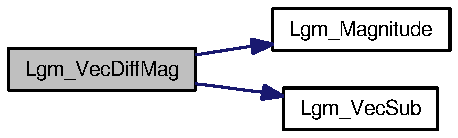
\includegraphics[width=128pt]{_lgm___vec_8c_3e1cdd838a8f00a41c167e848f6decf5_cgraph}
\end{center}
\end{figure}
\hypertarget{_lgm___vec_8c_47c6f330f5c1228f812b005094b64dfd}{
\index{Lgm\_\-Vec.c@{Lgm\_\-Vec.c}!Lgm\_\-ForceMagnitude@{Lgm\_\-ForceMagnitude}}
\index{Lgm\_\-ForceMagnitude@{Lgm\_\-ForceMagnitude}!Lgm_Vec.c@{Lgm\_\-Vec.c}}
\subsubsection[{Lgm\_\-ForceMagnitude}]{\setlength{\rightskip}{0pt plus 5cm}void Lgm\_\-ForceMagnitude ({\bf Lgm\_\-Vector} $\ast$ {\em a}, \/  double {\em mag})}}
\label{_lgm___vec_8c_47c6f330f5c1228f812b005094b64dfd}




Definition at line 108 of file Lgm\_\-Vec.c.

Here is the call graph for this function:\nopagebreak
\begin{figure}[H]
\begin{center}
\leavevmode
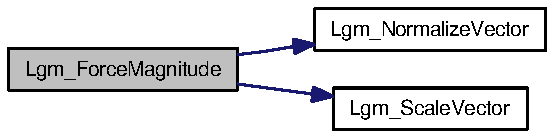
\includegraphics[width=151pt]{_lgm___vec_8c_47c6f330f5c1228f812b005094b64dfd_cgraph}
\end{center}
\end{figure}
\hypertarget{_lgm___vec_8c_d6b4ead73e36f4f3f77cc62bc88555d3}{
\index{Lgm\_\-Vec.c@{Lgm\_\-Vec.c}!Lgm\_\-MatTimesVec@{Lgm\_\-MatTimesVec}}
\index{Lgm\_\-MatTimesVec@{Lgm\_\-MatTimesVec}!Lgm_Vec.c@{Lgm\_\-Vec.c}}
\subsubsection[{Lgm\_\-MatTimesVec}]{\setlength{\rightskip}{0pt plus 5cm}void Lgm\_\-MatTimesVec (double {\em A}\mbox{[}3\mbox{]}\mbox{[}3\mbox{]}, \/  {\bf Lgm\_\-Vector} $\ast$ {\em V}, \/  {\bf Lgm\_\-Vector} $\ast$ {\em Result})}}
\label{_lgm___vec_8c_d6b4ead73e36f4f3f77cc62bc88555d3}




Definition at line 120 of file Lgm\_\-Vec.c.\hypertarget{_lgm___vec_8c_f287f148b722a2622150934c23fa59d4}{
\index{Lgm\_\-Vec.c@{Lgm\_\-Vec.c}!Lgm\_\-Transpose@{Lgm\_\-Transpose}}
\index{Lgm\_\-Transpose@{Lgm\_\-Transpose}!Lgm_Vec.c@{Lgm\_\-Vec.c}}
\subsubsection[{Lgm\_\-Transpose}]{\setlength{\rightskip}{0pt plus 5cm}void Lgm\_\-Transpose (double {\em A}\mbox{[}3\mbox{]}\mbox{[}3\mbox{]}, \/  double {\em B}\mbox{[}3\mbox{]}\mbox{[}3\mbox{]})}}
\label{_lgm___vec_8c_f287f148b722a2622150934c23fa59d4}




Definition at line 129 of file Lgm\_\-Vec.c.

Here is the caller graph for this function:\nopagebreak
\begin{figure}[H]
\begin{center}
\leavevmode
\includegraphics[width=258pt]{_lgm___vec_8c_f287f148b722a2622150934c23fa59d4_icgraph}
\end{center}
\end{figure}
\hypertarget{_lgm___vec_8c_cc29cb583eff692c2df92d9a49f3ce9e}{
\index{Lgm\_\-Vec.c@{Lgm\_\-Vec.c}!Lgm\_\-MatTimesMat@{Lgm\_\-MatTimesMat}}
\index{Lgm\_\-MatTimesMat@{Lgm\_\-MatTimesMat}!Lgm_Vec.c@{Lgm\_\-Vec.c}}
\subsubsection[{Lgm\_\-MatTimesMat}]{\setlength{\rightskip}{0pt plus 5cm}void Lgm\_\-MatTimesMat (double {\em A}\mbox{[}3\mbox{]}\mbox{[}3\mbox{]}, \/  double {\em B}\mbox{[}3\mbox{]}\mbox{[}3\mbox{]}, \/  double {\em R}\mbox{[}3\mbox{]}\mbox{[}3\mbox{]})}}
\label{_lgm___vec_8c_cc29cb583eff692c2df92d9a49f3ce9e}




Definition at line 148 of file Lgm\_\-Vec.c.

Here is the caller graph for this function:\nopagebreak
\begin{figure}[H]
\begin{center}
\leavevmode
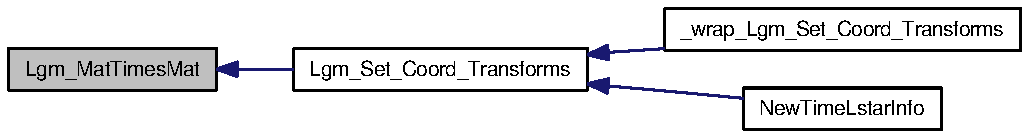
\includegraphics[width=265pt]{_lgm___vec_8c_cc29cb583eff692c2df92d9a49f3ce9e_icgraph}
\end{center}
\end{figure}
